\documentclass[11pt,
			   %10pt, 
               %hyperref={colorlinks},
               aspectratio=169,
               hyperref={colorlinks}
               ]{beamer}
\usetheme{Singapore}
\usecolortheme[snowy, cautious]{owl}

\usepackage[utf8]{inputenc}
\usepackage[T1]{fontenc}
\usepackage[american]{babel}
\usepackage{graphicx}
\usepackage{hyperref}

\hypersetup{
    colorlinks=true,
    urlcolor=[rgb]{1,0,1},
    linkcolor=[rgb]{1,0,1}}
\definecolor{magenta}{RGB}{255, 0, 255}

\usepackage[natbib=true,style=numeric,backend=bibtex,useprefix=true]{biblatex}

\definecolor{OwlGreen}{RGB}{75,0,130} % easier to see
\setbeamertemplate{bibliography item}{\insertbiblabel}
\setbeamerfont{caption}{size=\footnotesize}
\setbeamertemplate{frametitle continuation}{}

\setcounter{tocdepth}{1}
\renewcommand*{\bibfont}{\scriptsize}
\addbibresource{bibliography.bib}

\renewcommand*{\thefootnote}{\fnsymbol{footnote}}

\usenavigationsymbolstemplate{}
\setbeamertemplate{footline}{%
    \raisebox{5pt}{\makebox{\hfill\makebox[20pt]{\color{gray}
          \scriptsize\insertframenumber}}}\hspace*{5pt}}

\usepackage{epigraph}
% \epigraphsize{\small}% Default
\setlength\epigraphwidth{14cm}
\setlength\epigraphrule{0pt}
\usepackage{etoolbox}
\makeatletter
\patchcmd{\epigraph}{\@epitext{#1}}{\itshape\@epitext{#1}}{}{}
\makeatother

\author{\copyright\hspace{1pt}Patrick Hall\footnote{\tiny{This material is shared under a \href{https://creativecommons.org/licenses/by/4.0/deed.ast}{CC By 4.0 license} which allows for editing and redistribution, even for commercial purposes. However, any derivative work should attribute the author and H2O.ai.}}}
\title{Guidelines for Responsible Use of Explainable Machine Learning}
\logo{
\includegraphics[height=8pt]{img/h2o_logo.png}}
\institute{\href{https://www.h2o.ai}{H\textsubscript{2}O.ai}}
\date{\today}
\subject{}

\begin{document}
	
	\maketitle
	
	\begin{frame}
	
		\frametitle{Contents}
		
		\tableofcontents{}
		
	\end{frame}

%-------------------------------------------------------------------------------
	\section{Introduction}
%-------------------------------------------------------------------------------

%-------------------------------------------------------------------------------
	\subsection{What?}
%-------------------------------------------------------------------------------

	\begin{frame}[t]
		
		\frametitle{What is explainable machine learning (ML)?}
		
		\epigraph{“A collection of visual and/or interactive artifacts that provide a user with sufficient description of the model behavior to accurately perform tasks like evaluation, trusting, predicting, or improving the model.”}{--- \textup{Sameer Singh}, UCI}		
		
		\scriptsize Variously defined along with aliases or similar concepts:
		\begin{itemize}\scriptsize
			\item ``Towards a Rigorous Science of Interpretable Machine Learning'' (\citet{been_kim1})
			\item ``Explaining Explanations'' (\citet{gilpin2018explaining})
			\item ``A Survey Of Methods For Explaining Black Box Models'' (\citet{guidotti2018survey})
			\item ``The Mythos of Model Interpretability'' (\citet{lipton1})
		 	\item \textit{Interpretable Machine Learning} (\citet{molnar})
			\item ``Interpretable Machine Learning: Definitions, Methods, and Applications'' (\citet{murdoch2019interpretable})
			\item ``Challenges for Transparency'' (\citet{weller2017challenges}). 
		\end{itemize}\normalsize
		
	\end{frame}
	
	\begin{frame}
	
		\frametitle{What is explainable ML?}

		What do \textit{\textbf{I}} mean by explainable ML?\\
		\vspace{5pt}
		Mostly post-hoc techniques used to enhance \textit{\textbf{understanding}} of trained model mechansims and predictions, e.g. ...
		\begin{itemize}
			\item \textbf{Direct measures of global and local feature importance}: 
			\begin{itemize}\footnotesize
				\item Gradient-based feature attribution (\citet{grad_attr})
				\item Shapley values (\citet{shapley})
			\end{itemize}
			\item \textbf{Global and local surrogate models}: 
			\begin{itemize}\footnotesize
				\item Decision tree variants (\citet{viper}, \citet{dt_surrogate1})
				\item Anchors (\citet{anchors})
				\item Local interpretable model-agnostic explanations (LIME) (\citet{lime})
			\end{itemize}
			\item \textbf{Global and local visualizations of trained model predictions}: 
			\begin{itemize}\footnotesize
				\item Accumulated local effect (ALE) (\citet{ale_plot}) 
				\item Partial dependence (\citet{esl})
				\item Individual conditional expectation (ICE) (\citet{ice_plots})
			\end{itemize}
		\end{itemize}\normalsize
			
	\end{frame}
	
%-------------------------------------------------------------------------------
	\subsection{Why?}
%-------------------------------------------------------------------------------

% ask for contributions to awesome-machine-learning-interpretability

	\begin{frame}
	
		\frametitle{Why explainable ML?}
		\vspace{10pt}
		Responsible Use of Explainable ML can enable:
		\begin{itemize}\footnotesize
			\item Human learning from machine learning
			\item Human appeal of automated decisions
			\item Regulatory compliance
			\item White-hat/red-team hacking
		\end{itemize}
		\vspace{5pt}
		Misuse and Abuse of Explainable ML can enable:
		\begin{itemize}\footnotesize
			\item Model and data stealing (\citet{model_stealing}, \citet{membership_inference}, \citet{shokri2019privacy})
			\item False justification for harmful black-boxes, e.g. ``fairwashing'' (\citet{fair_washing}, \citet{please_stop})
		\end{itemize}
		\normalsize
		
	\end{frame}
	
% regulation?	
	
%-------------------------------------------------------------------------------
	\subsection{Guidelines}
%-------------------------------------------------------------------------------	

	\begin{frame}
	
		\frametitle{Proposed Guidelines for Responsible Use}
		
		Explainable ML is already in-use: numerous open source\footnote{\tiny{See: \url{https://github.com/jphall663/awesome-machine-learning-interpretability}}} and commercial packages\footnote{\tiny{For instance  Datarobot, H2O Driverless AI, SAS Visual Data Mining and Machine Learning, Zest AutoML}} are available today.\\
		\vspace{5pt}
		Best-practices are needed to prevent misuse and abuse. So, four basic guidelines are proposed here:
		\vspace{5pt}
		\begin{itemize}
			\item Use explainable ML to enhance understanding.
			\item Learn how explainable ML is used for nefarious purposes.
			\item Augment surrogate models with direct explanations.
			\item Use highly transparent mechanisms for high stakes applications.
		\end{itemize}
		
	\end{frame}

%-------------------------------------------------------------------------------
	\section{Understanding and Trust}
%-------------------------------------------------------------------------------

	\begin{frame}
	
		\frametitle{Use Explainable ML to Enhance Understanding.}
		
		Explanations enhance understanding directly, and increase trust as a side-effect.\\
		\vspace{10pt}
		Models can be understood and not trusted, and trusted but not understood.\\
		\vspace{10pt}
		Explanations alone are neither necessary nor sufficient for trust.
		
	\end{frame}

	\begin{frame}[label={no_trust}]
	
		\frametitle{Understanding Without Trust}
		
					\begin{columns}
				
						\column{0.5\linewidth}
						\centering
						\vspace{7pt}\\
						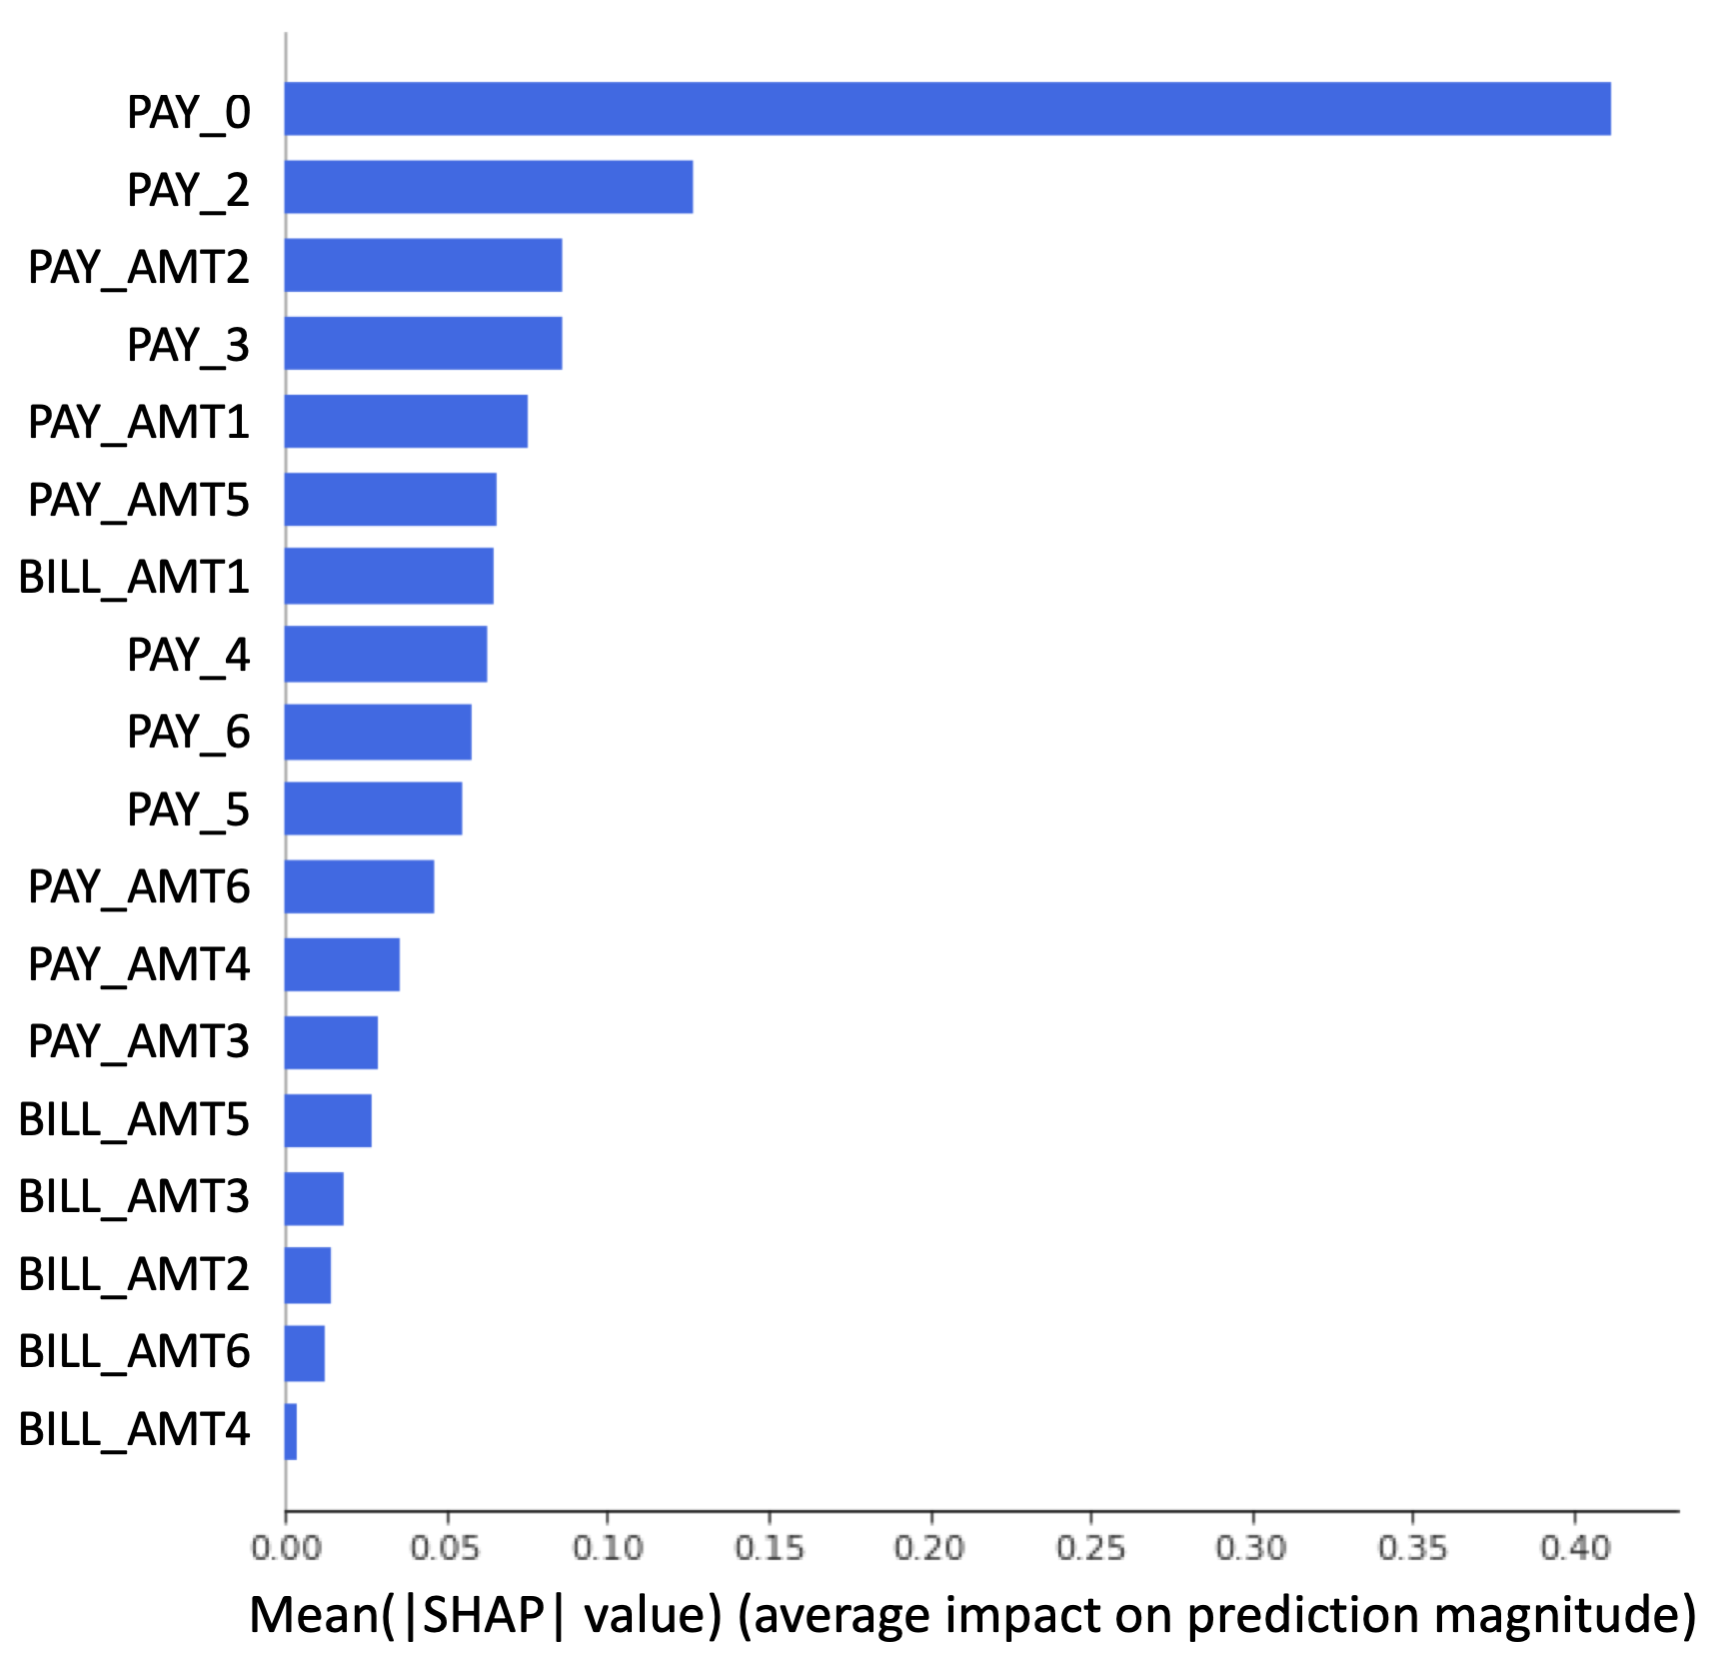
\includegraphics[height=140pt]{img/global_shap.png}\\
						\vspace{5pt}
						\tiny{$g_{\text{mono}}$ monotonically-constrained probability of default (PD) classifier trained on the UCI credit card dataset over-emphasizes the most important feature, a customer's most recent repayment status, $\text{PAY\_0}$ \cite{uci}.}

						\vspace{10pt}
						\column{0.6\linewidth}
						\centering
						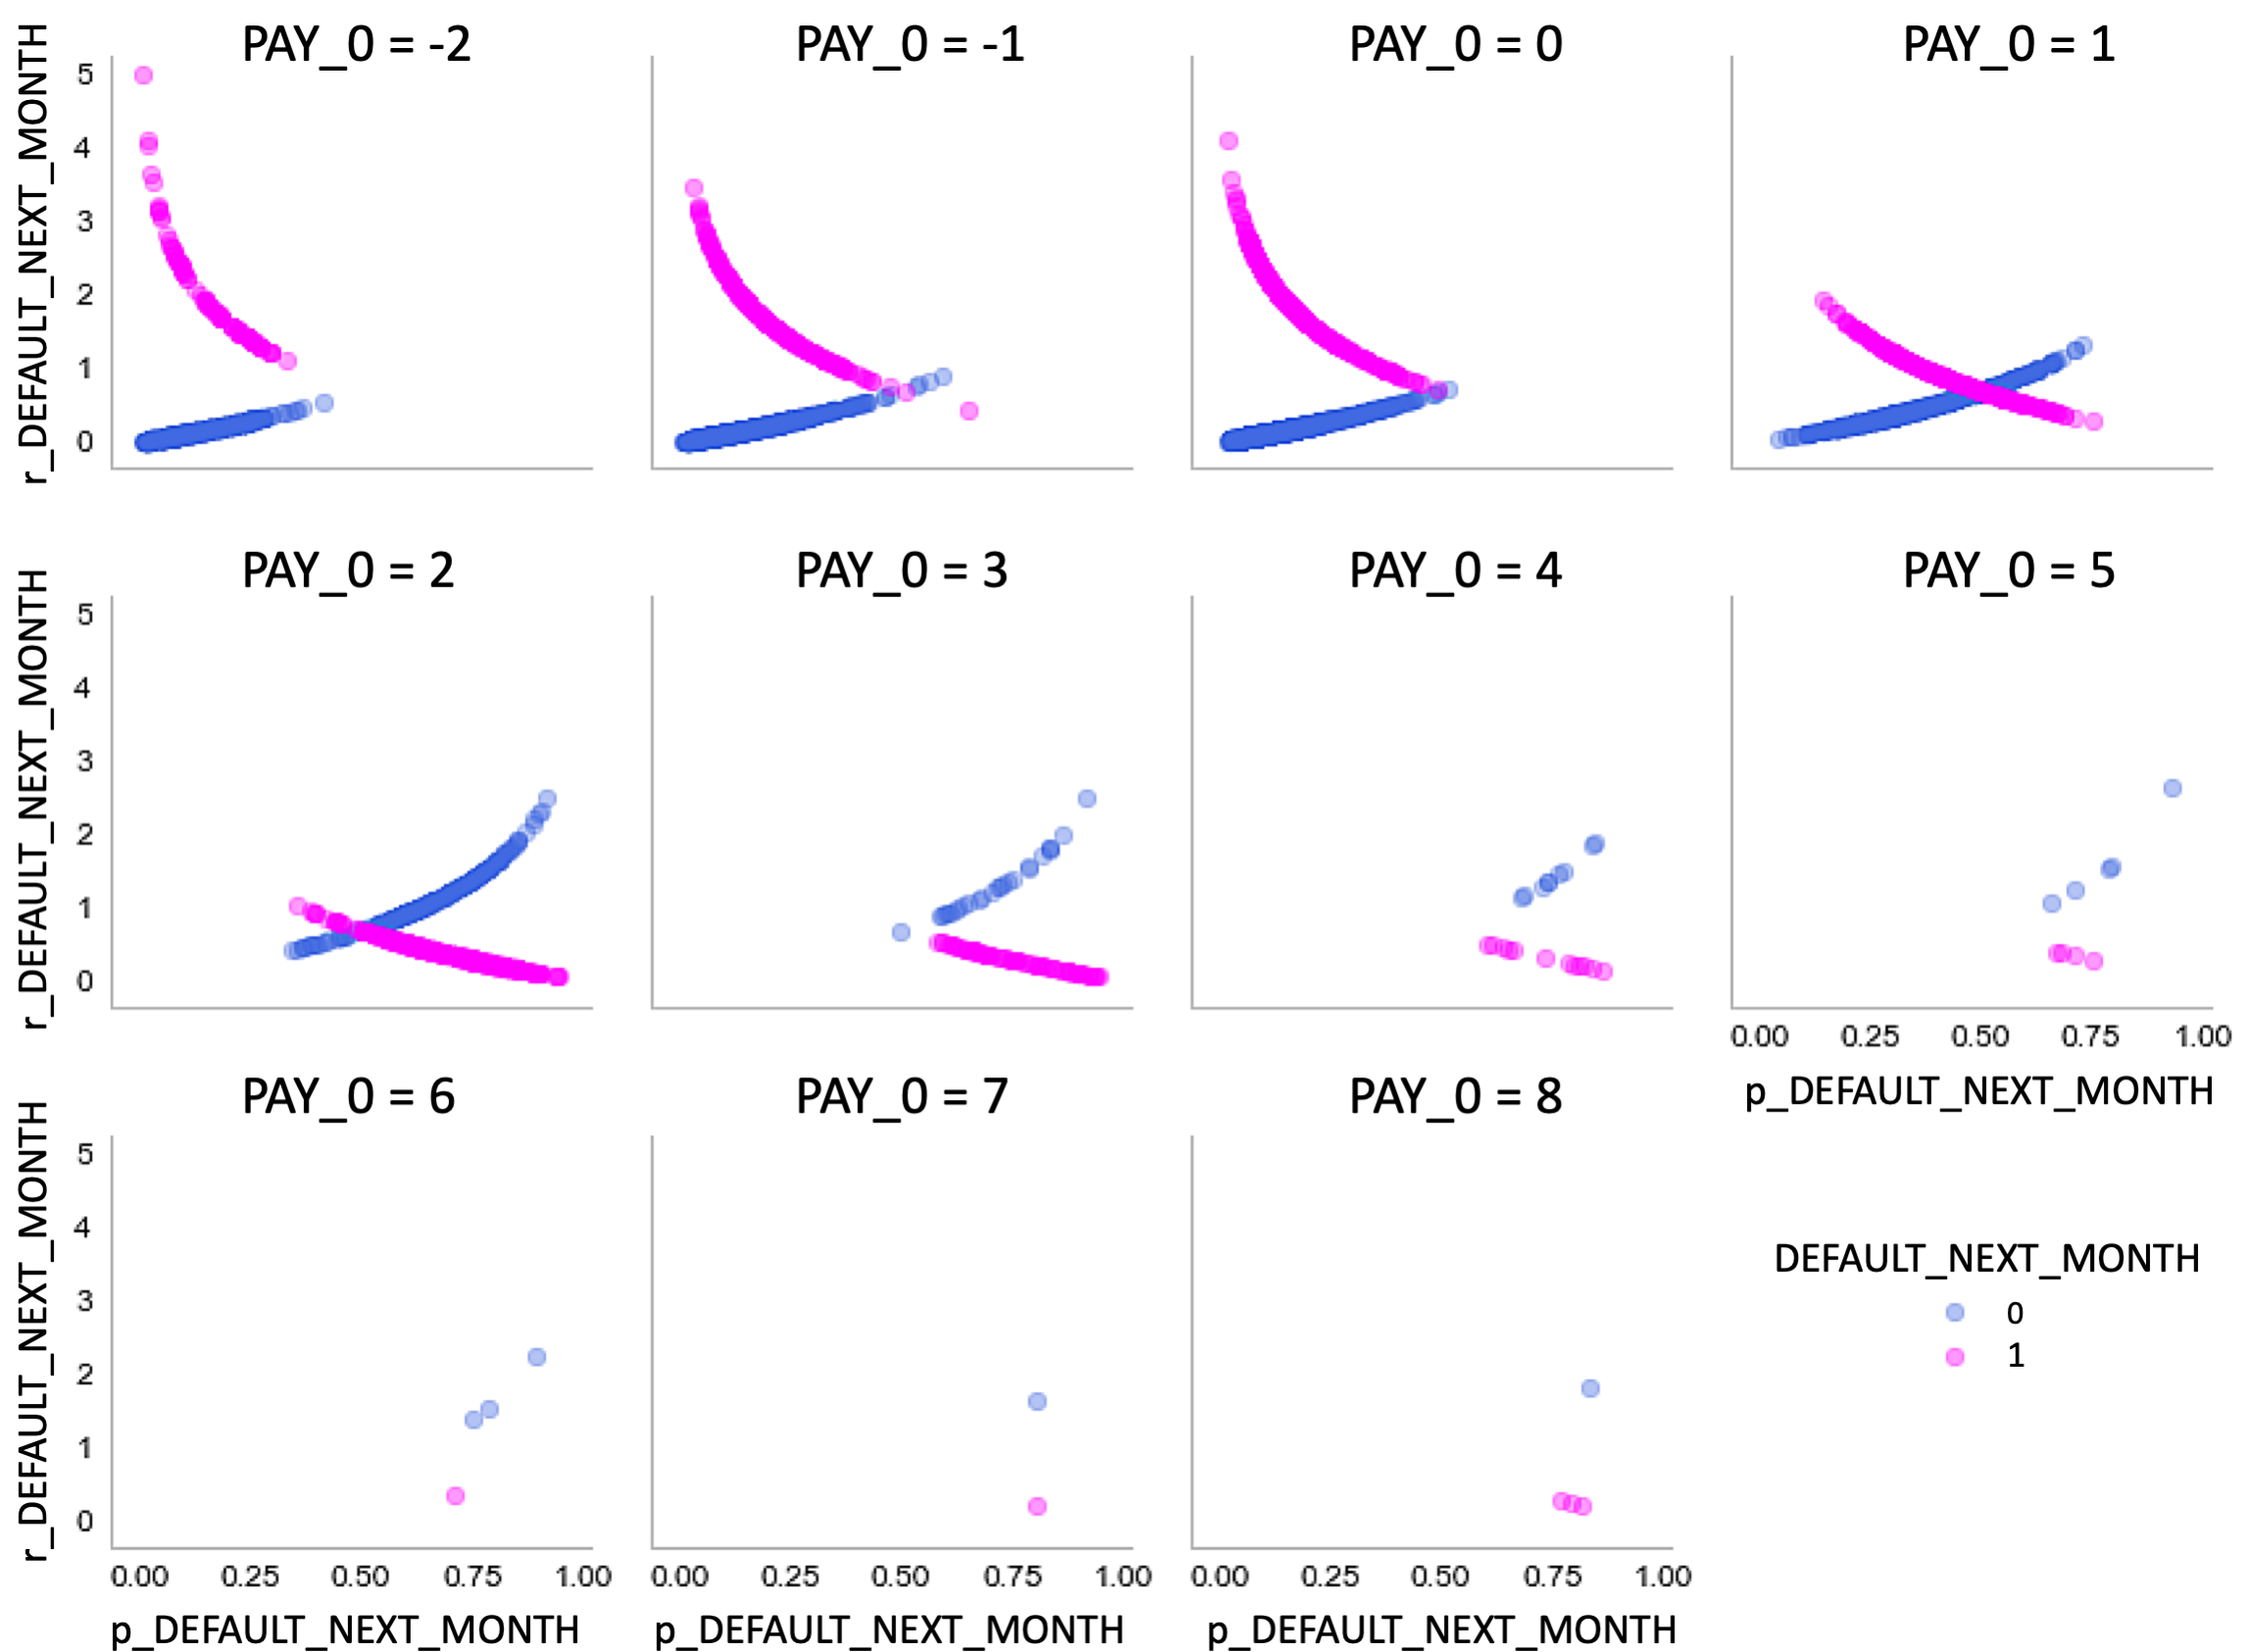
\includegraphics[height=130pt]{img/resid.png}\\
						\vspace{5pt}
						\tiny{$g_{\text{mono}}$ also struggles to predict default for favorable statuses, $-2  \leq \texttt{PAY\_0}  < 2$, and often cannot predict on-time payment when recent payments are late, $\text{PAY\_0} \geq 2$}.
				
					\end{columns}
					\normalsize				
		
	\end{frame}
	
	\begin{frame}
	
		\frametitle{Trust Without Understanding}
		
		Years before reliable explanation techniques were widely acknowledged and available, black-box predictive models, such as autoencoder and MLP neural networks, were used for fraud detection in the financial services industry \cite{gopinathan1998fraud}. When these models performed well, they were trusted.\footnote{For example: \url{https://www.sas.com/en_ph/customers/hsbc.html}, \url{https://www.kdnuggets.com/2011/03/sas-patent-fraud-detection.html}.} However, they were not explainable or well-understood by contemporary standards.  

	\end{frame}


%-------------------------------------------------------------------------------
	\section{The Dark Side}
%-------------------------------------------------------------------------------

	\begin{frame}
	
		\frametitle{Learn How Explainable ML is Used for Nefarious Purposes}	
		
		When unintentionally misused, explainable ML can act as a faulty-safeguard for a potentially harmful black-box.\\
		\vspace{10pt}
		When intentionally abused, explainable ML can be used for: 
		\begin{itemize}
			\item Hacking of data, models, or other intellectual property.
			\item \textit{Fairwashing}, to mask the sociological biases of a discriminatory black-box.
		\end{itemize}
	
	\end{frame}


	\begin{frame}
	
		\frametitle{ML Hacking}
		
\footnotesize{Many ML hacks use, or are exacerbated by, explainable ML techniques.}\footnote{\tiny{See \url{https://github.com/jphall663/secure_ML_ideas} for full size image and more information.}}
				\begin{figure}
					\begin{center}
						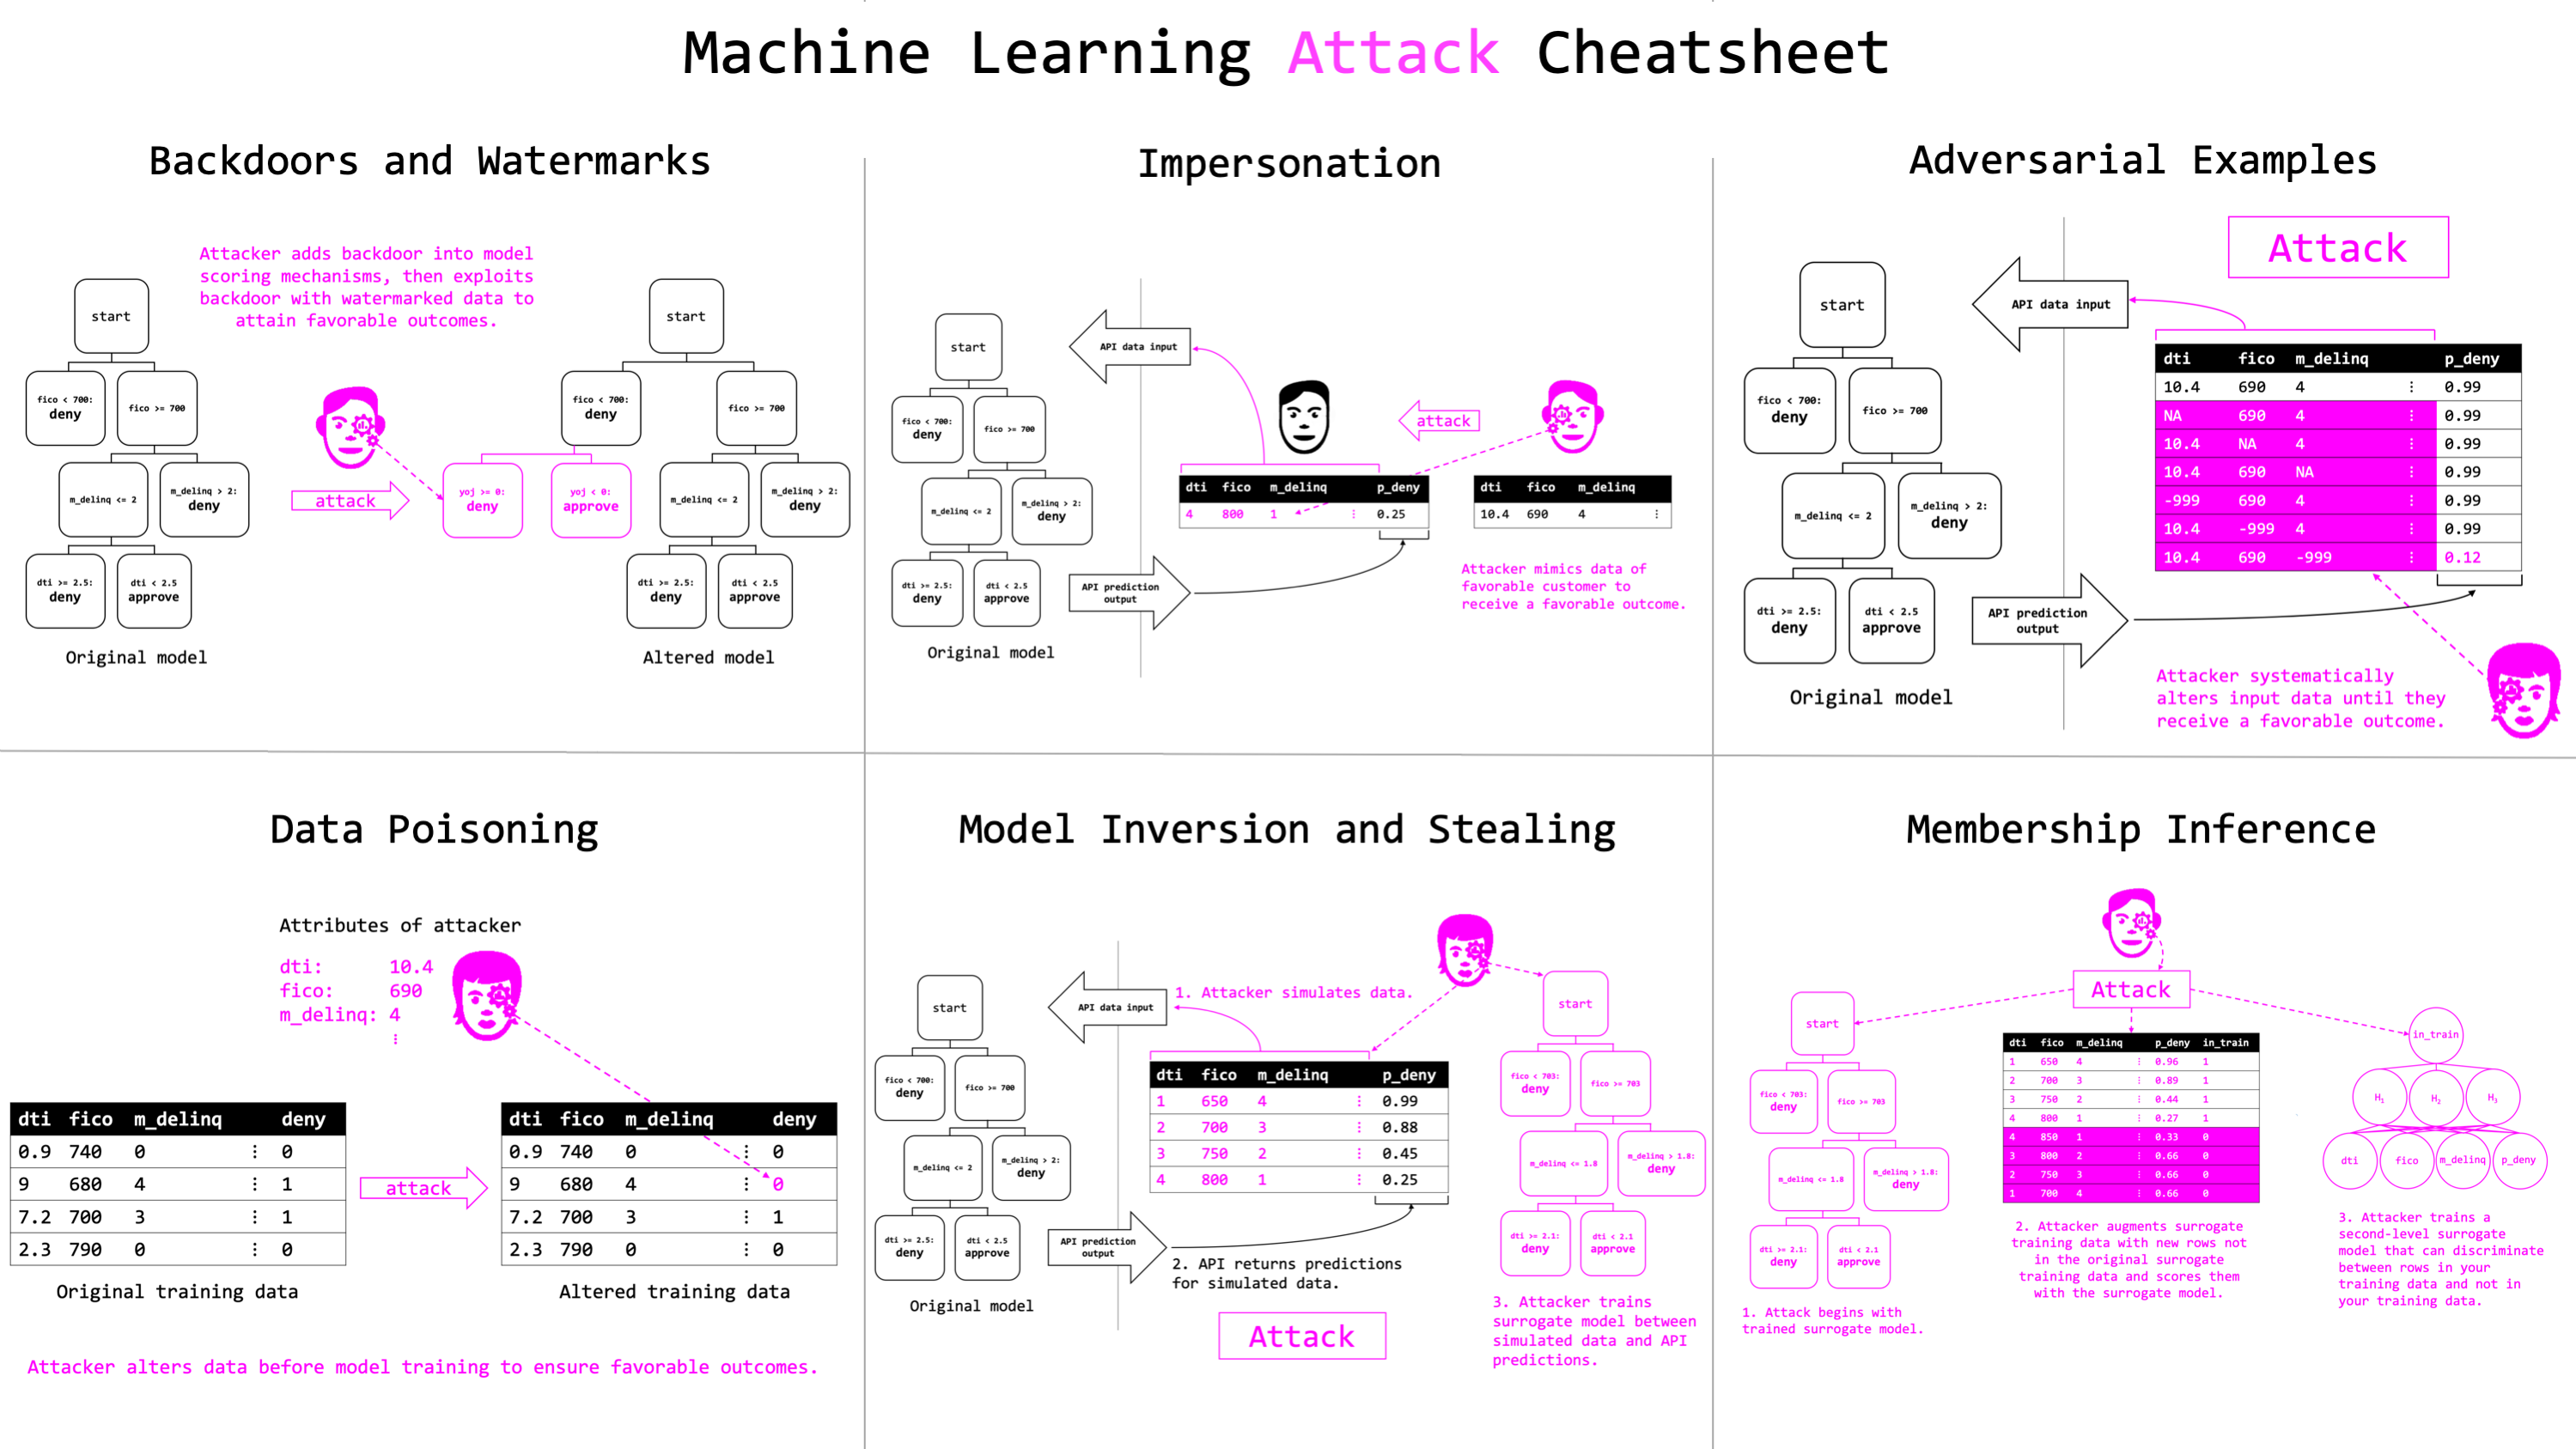
\includegraphics[height=160pt]{img/cheatsheet.png}
					\end{center}
				\end{figure}	
				\normalsize
	
	\end{frame}
	
	\begin{frame}
	
		\frametitle{White-hat Attacks}
		
		The flip-side of the dark side is community oversight of black-boxes.\\
		\vspace{10pt}
		Recent high profile analyses of commercial black-boxes, \href{https://www.propublica.org/article/machine-bias-risk-assessments-in-criminal-sentencing}{Propublica and COMPAS} and \href{https://medium.com/@Joy.Buolamwini/response-racial-and-gender-bias-in-amazon-rekognition-commercial-ai-system-for-analyzing-faces-a289222eeced}{Gendershades and Rekognition}, can be viewed as white-hat attacks (model stealing, adversarial examples) on proprietary black-boxes.\footnote{This presentation makes no claim on the quality of the analysis in Angwin et al. (2016), which has been criticized, but is simply stating that such cracking is possible \cite{angwin16,}, \cite{flores2016false}.} 

	\end{frame}
	
	\begin{frame}[label={not_frontline}]
	
		\frametitle{Explanation \textbf{\textit{is Not}} a Front Line Fairness Tool}
		
		Use fairness tools, e.g. ...
		\vspace{5pt}
		\begin{itemize}\footnotesize
			\item Disparate impact testing (\citet{feldman2015certifying})
			\item Reweighing (\citet{kamiran2012data})
			\item Reject option based classification (\citet{kamiran2012decision})
			\item Adversarial de-biasing (\citet{zhang2018mitigating})
			\item \href{https://github.com/dssg/aequitas}{aequitas}, \href{https://github.com/IBM/AIF360}{AIF360}, \href{https://github.com/LASER-UMASS/Themis}{Themis}, \href{https://github.com/cosmicBboy/themis-ml}{themis-ml}
		\end{itemize}
		\vspace{5pt}
		... for fairness tasks: bias testing, bias remediation, and to establish trust.\\
		\vspace{10pt}
		Explanations can be used to understand and augment such results.
		
	\end{frame}
	
%-------------------------------------------------------------------------------
	\section{Surrogates}
%-------------------------------------------------------------------------------

	\begin{frame}
	
		\frametitle{Surrogate Models}
		
		Models of models, or surrogate models, can be helpful explanatory or modeling tools, but they are usually approximate, low-fidelity explainers.\\
		\vspace{10pt}
		Much work in explainable ML has been directed toward improving the fidelity and usefulness of surrogate models (e.g., \citet{dt_surrogate2}, \citet{viper}, \citet{dt_surrogate1}, \citet{lime-sup}, \citet{wf_xnn})\\
		\vspace{10pt}
		\textbf{\textit{Many explainable ML techniques have nothing to do with surrogate models!}}
		
	\end{frame}
	
	\begin{frame}[t]
	
		\frametitle{Augment Surrogate Models with Direct Explanations}	
	
		\begin{columns}
				
			\column{0.55\linewidth}
			\centering			
			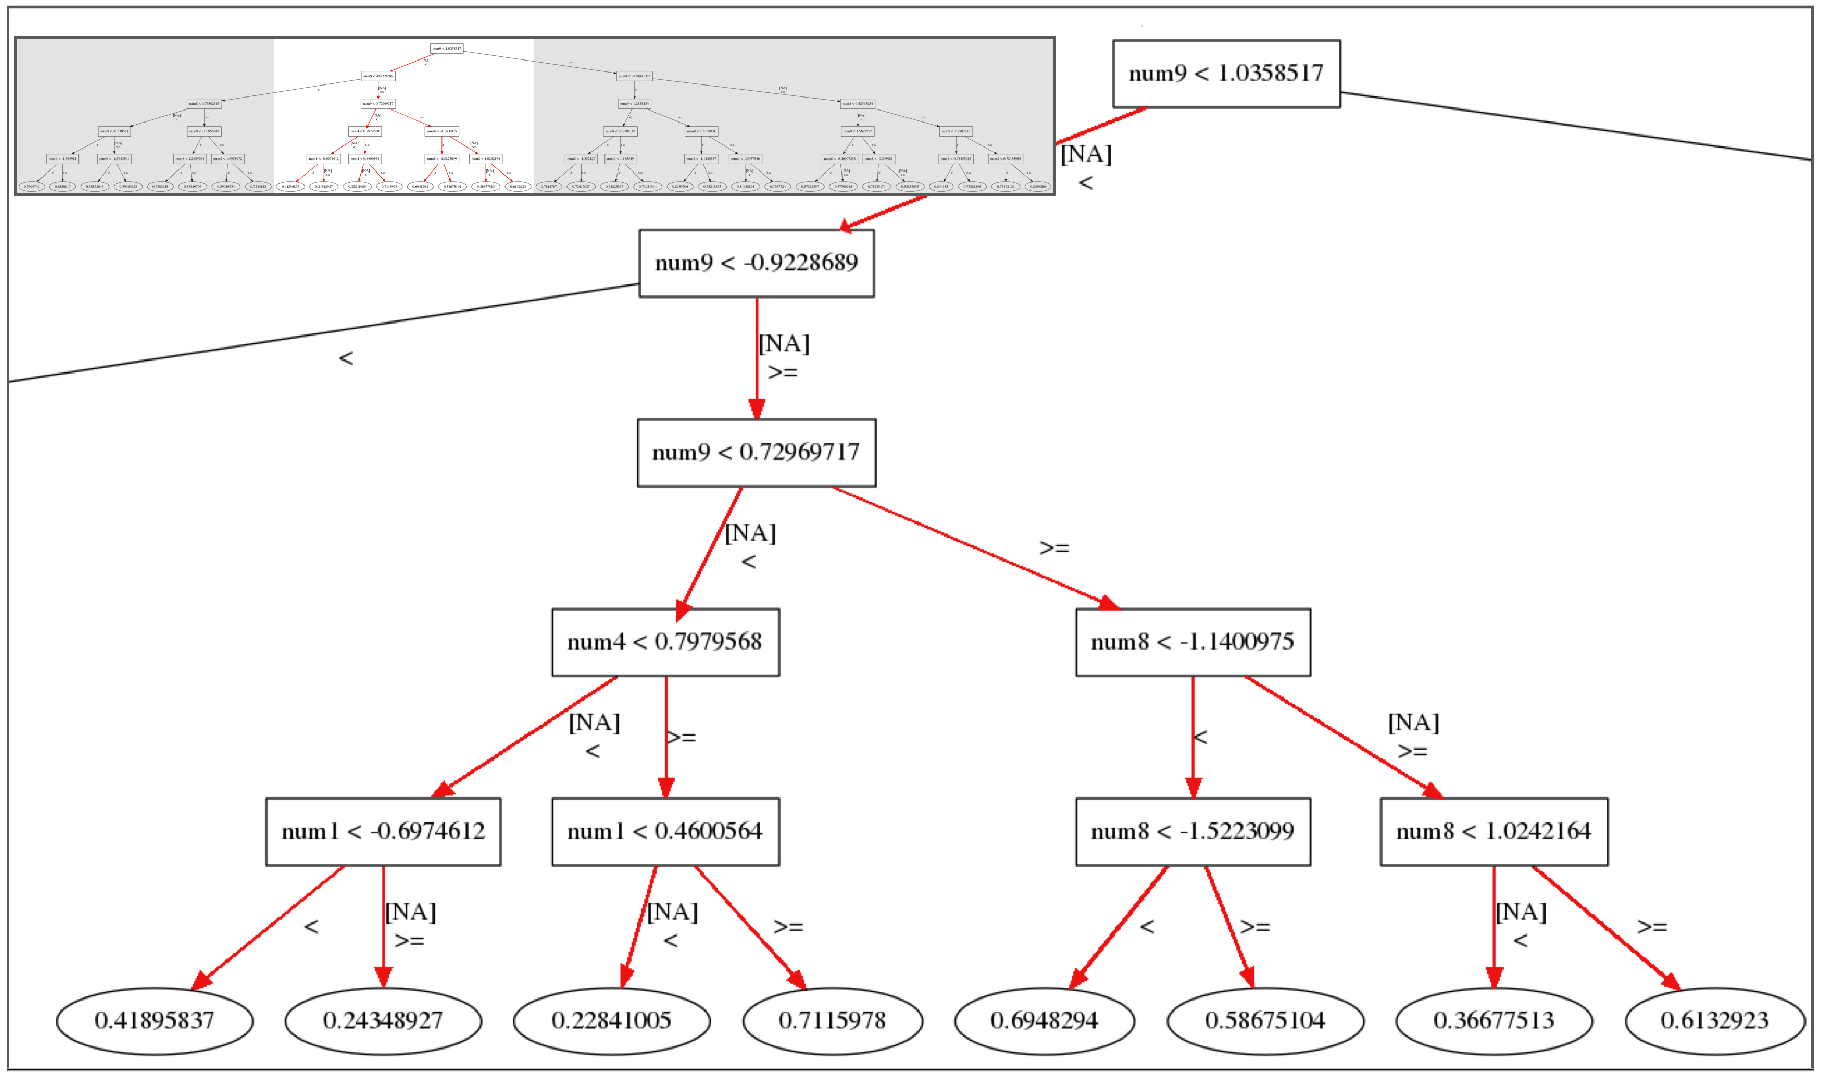
\includegraphics[height=0.6\linewidth, width=.95\linewidth]{img/figure_3-eps-converted-to.pdf}\\
  			\tiny{Na\"ive $h_{\text{tree}}$, \textit{a surrogate model}, forms an approximate overall flowchart for the explained model, $g_{\text{GBM}}$.}

			\hspace{5pt}
			\column{.45\textwidth}
  			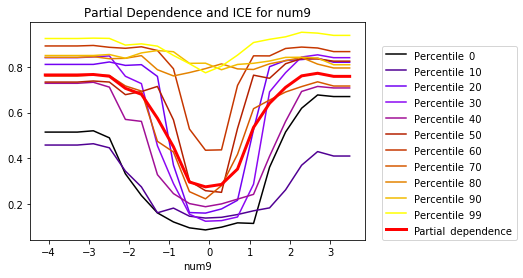
\includegraphics[height=.52\linewidth, width=1.02\linewidth]{img/figure_4.png}\\
  			\tiny{Partial dependence and ICE curves generated \textit{directly from the explained model}, $g_{\text{GBM}}$.}
  			
  		\end{columns}

	\scriptsize{$h_{\text{tree}}$ displays known interactions in $f = X_{\text{num}1} * X_{\text{num}4} + |X_{\text{num}8}| * X_{\text{num}9}^2$ for $\sim -0.923 < X_{\text{num9}} <  \sim 1.04$. Modeling of the known interaction between $X_{\text{num9}}$ and $X_{\text{num8}}$ in $f$ by $g_{\text{GBM}}$ is confirmed by the divergence of partial dependence and ICE curves for $\sim -1 < X_{\text{num9}} <  \sim 1$.}

	\end{frame}

	\begin{frame}[t, label={lime}]
	
		\frametitle{Augment LIME with Direct Explanations}
	
		\begin{columns}
				
			\column{0.5\linewidth}
			\centering			
			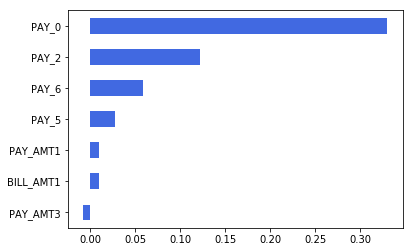
\includegraphics[height=0.6\linewidth, width=.95\linewidth]{img/shap.png}\\
  			\tiny{Locally-accurate Shapley contributions for a high risk individual's probability of default as predicted by a simple decision tree model, $g_{\text{tree}}$. See slide~\ref{dt} for a directed graph representation of $g_{\text{tree}}$}.

			\hspace{5pt}
			\column{0.5\linewidth}
			\begin{table}
				\centering
				\tiny
				\begin{tabular}{ | p{2cm} | p{1.7cm} | }
					\hline
					$h_{\text{GLM}}$\newline Feature & $h_{\text{GLM}}$\newline Coefficient \\ 
					\hline
					\texttt{PAY\_0 == 4} & $0.0009$ \\
					\hline
					\texttt{PAY\_2 == 3} & $0.0065$ \\
					\hline
					\texttt{PAY\_5 == 2} & $-0.0006$ \\
					\hline
					\texttt{PAY\_6 == 2} & $0.0036$ \\
					\hline				
					\texttt{BILL\_AMT1} & $3.4339\mathrm{e}{-08}$ \\
					\hline
					\texttt{PAY\_AMT1} & $4.8062\mathrm{e}{-07}$ \\
					\hline	
					\texttt{PAY\_AMT3} & $-5.867\mathrm{e}{-07}$ \\	
					\hline	
				\end{tabular}	
			\end{table}	
  			\tiny{Coefficients for a local linear interpretable model, $h_{\text{GLM}}$, with an intercept of 0.77 and an $R^2$ of 0.73., trained between the original inputs and predictions of $g_{\text{tree}}$ for a segment of the UCI credit card dataset with late most recent repayment statuses, $\mathbf{X}_{PAY \_ 0 > 1}$}.
  		\end{columns}

	\scriptsize{Because $h_{GLM}$ is relatively well-fit and has a logical intercept, it can be used along with Shapley values to reason about the modeled average behavior for risky customers and to differentiate the behavior of any one specific risky customer from their peers under the model.}

	\end{frame}


%-------------------------------------------------------------------------------
	\section{High Stakes Applications}
%-------------------------------------------------------------------------------

% regulation?

	\begin{frame}
	
		\frametitle{Use Highly Transparent Mechanisms for High Stakes Applications}	
		
		\centering{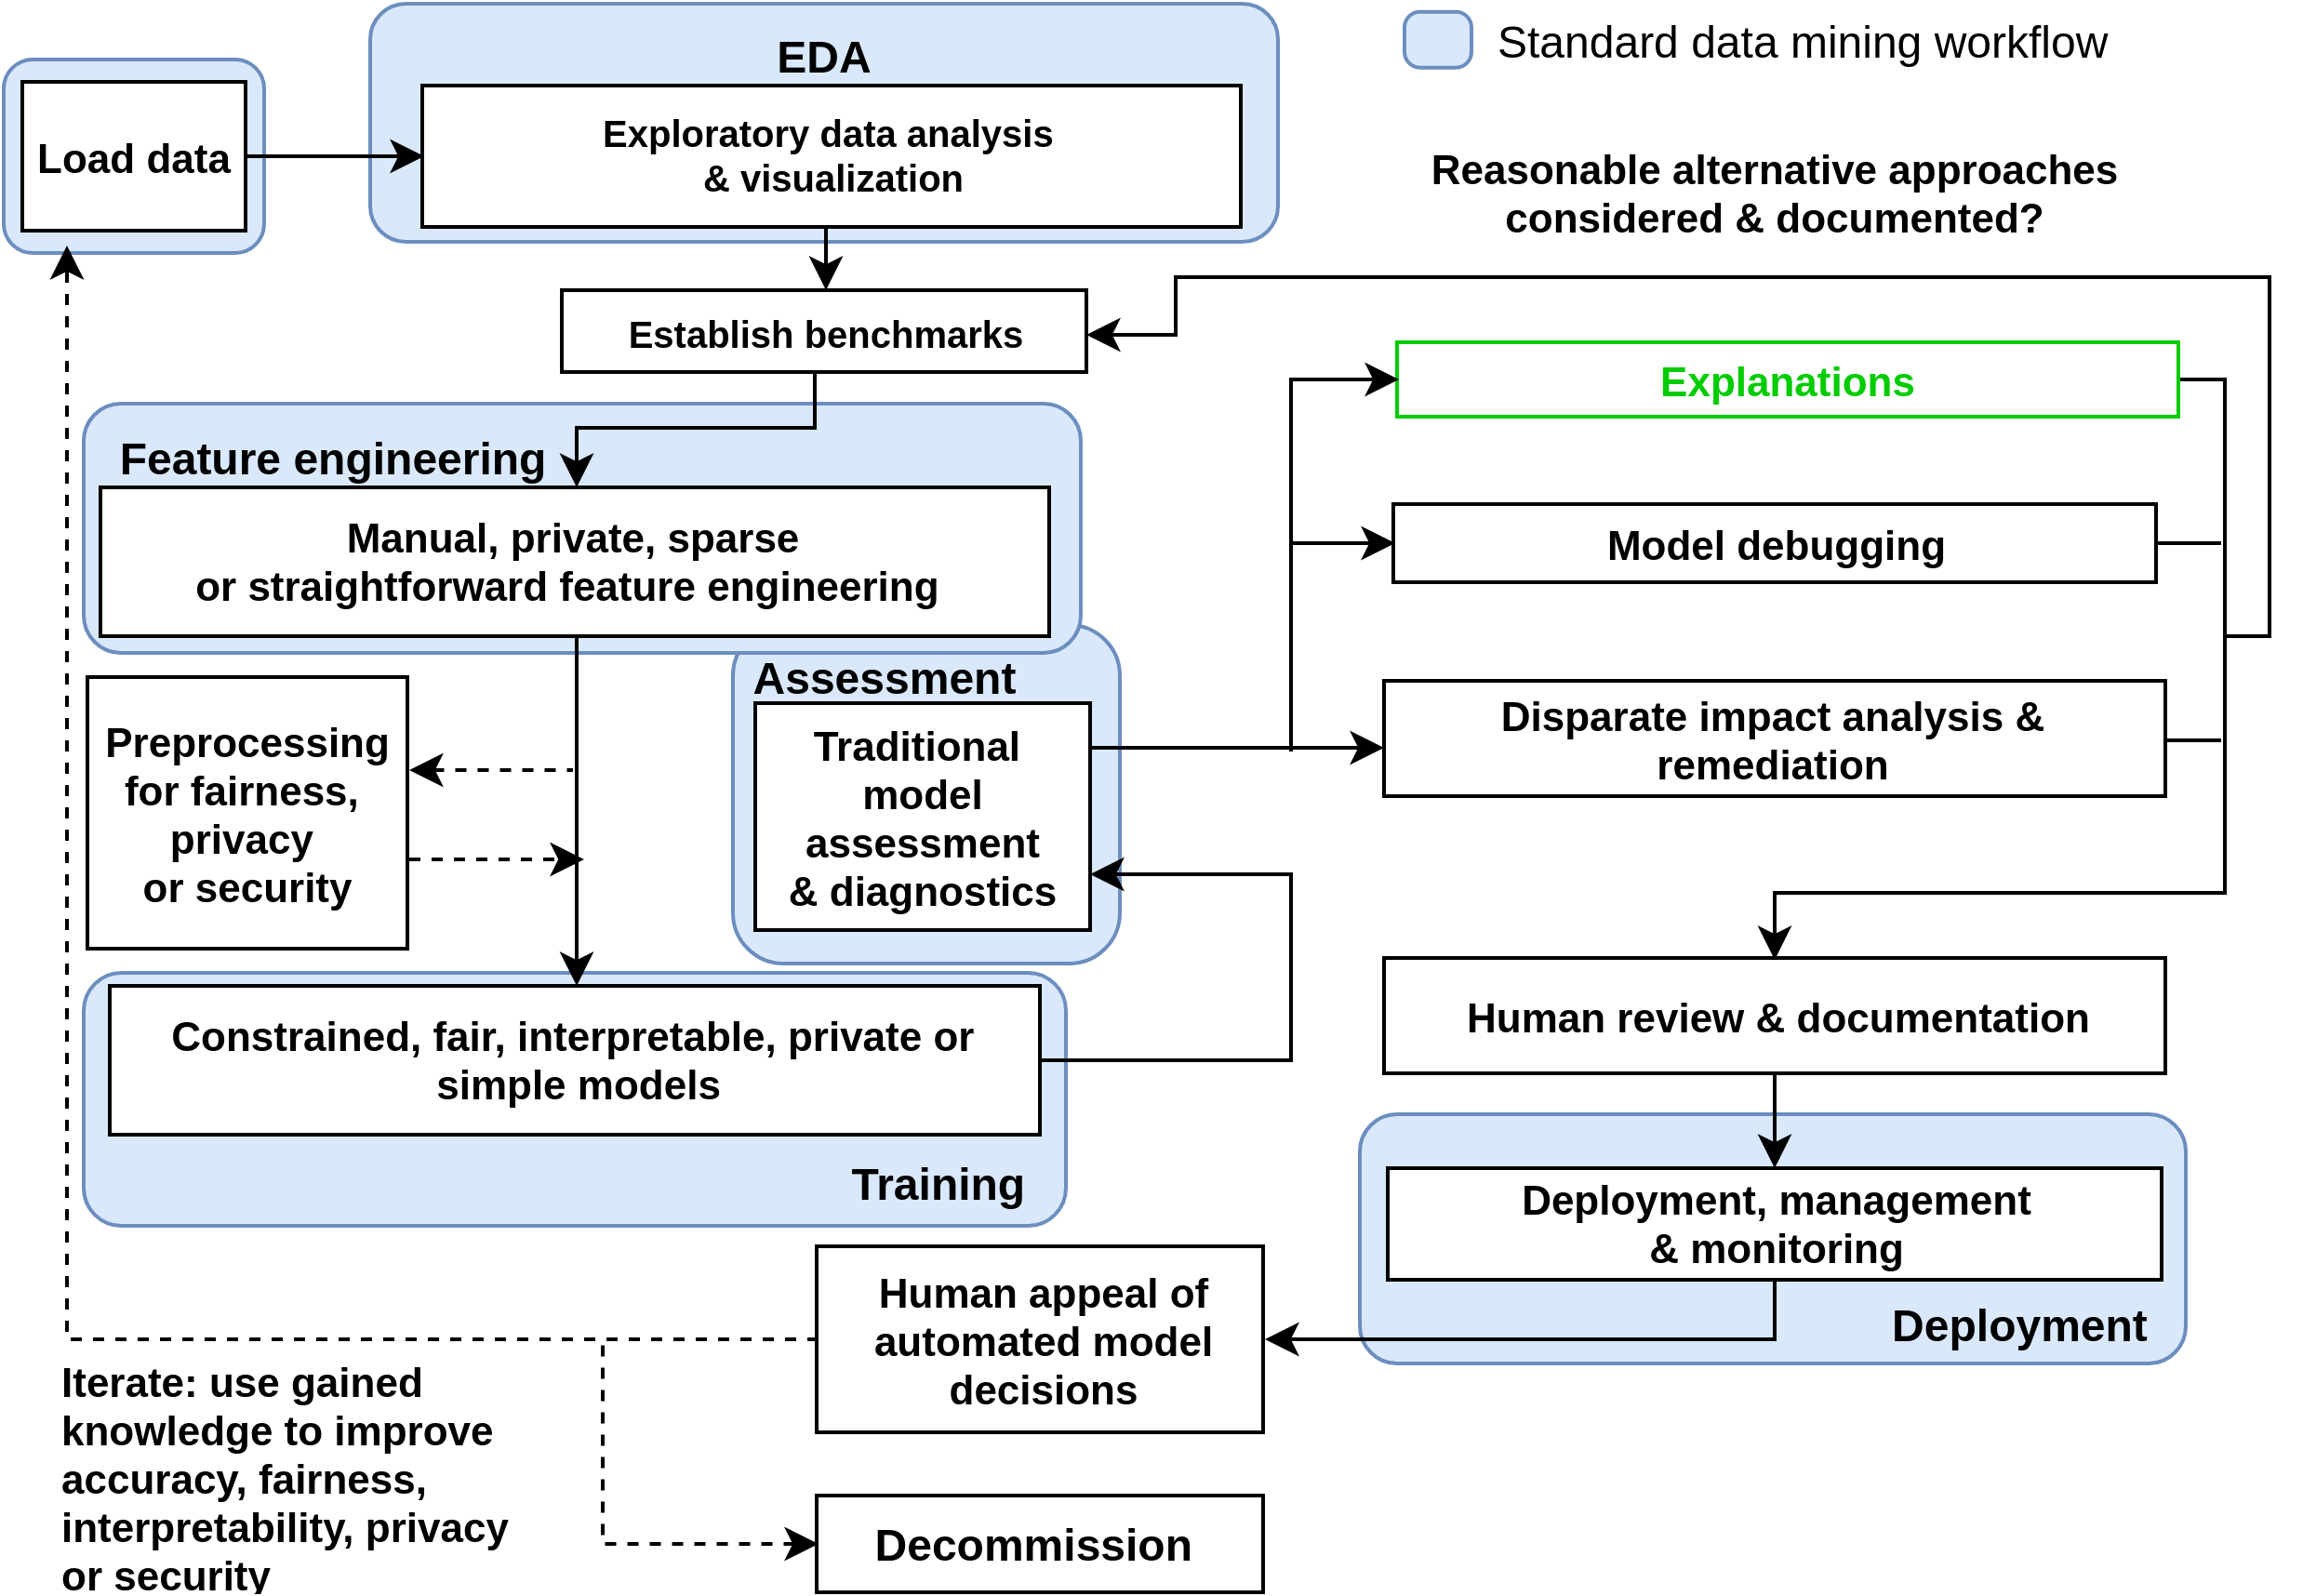
\includegraphics[scale=0.08]{img/figure_1_lo.png}}\\
		\vspace{5pt}
		\scriptsize{A diagram of a proposed low risk ML workflow in which explanations (highlighted in green) are used along with interpretable or white-box models, disparate impact analysis and remediation techniques, and other review and appeal mechanisms to create a fair, accountable, and transparent ML system.}
	
	\end{frame}

	\begin{frame}
	
		\frametitle{Interpretable Models}
		
		Many types of novel interpretable models are freely available today, e.g. 
		
		\begin{itemize}
			\item \href{https://github.com/microsoft/interpret}{Explainable boosting machine (EBM)}
			\item Monotonic GBM in \href{https://github.com/h2oai/h2o-3}{h2o} or \href{https://github.com/dmlc/xgboost}{XGBoost}
			\item \href{https://cran.r-project.org/web/packages/pre/index.html}{RuleFit} (\citet{rulefit})
			\item \href{https://github.com/ustunb/slim-python}{Super-sparse linear integer model} (SLIM)	(\citet{slim})
			\item \href{https://cran.r-project.org/web/packages/sbrl/index.html}{Scalable Bayesian rule list} (\citet{sbrl})

		
		\end{itemize}	
	
	\end{frame}	

% shades of interpretability

	\begin{frame}[label={dt}]
	
		\frametitle{Explanations and Interpretable Models are Not Mutually Exclusive}	
		
		\begin{columns}
				
			\column{0.5\linewidth}
			\centering		
			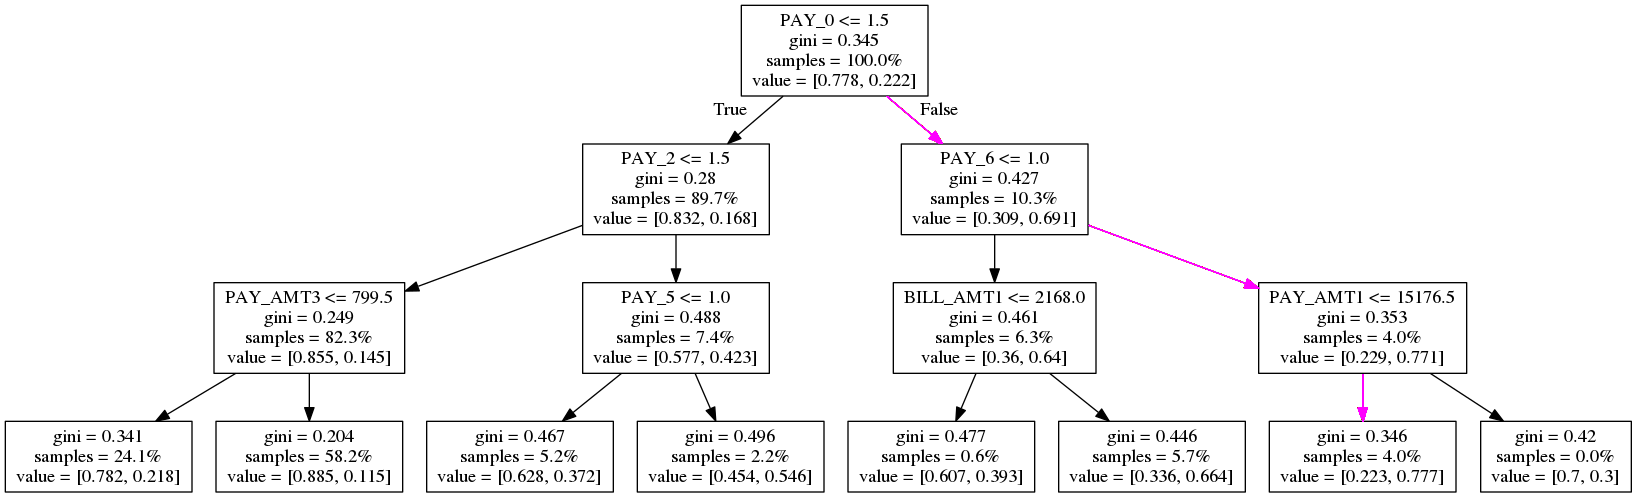
\includegraphics[height=.45\linewidth, width=1.15\linewidth]{img/dt.png}\\
			\vspace{5pt}
  			\tiny{Simple decision tree, $g_{\text{tree}}$, trained on the UCI credit card data to predict default with validation AUC of 0.74. The decision policy for a high risk individual is highlighted in red.}

			\hspace{50pt}
			\column{.4\textwidth}
			\centering
			\vspace{2pt}\\
  			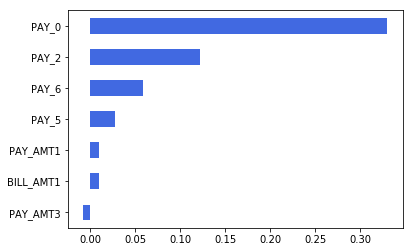
\includegraphics[height=.5\linewidth, width=.8\linewidth]{img/shap.png}\\
  			\vspace{5pt}
  			\tiny{Locally-accurate Shapley contributions for the highlighted individual's probability of default. See slide \ref{lime} for LIMEs for the high risk customers in $g_{\text{tree}}$.}

		\end{columns}
		\vspace{10pt}

	\scriptsize{The Shapley values are helpful because they highlight the local importance of features not on the decision path, which could be underestimated by examining the decision policy alone.}
	
	\end{frame}
	
	\begin{frame}
		
		\frametitle{An Ode to the Shapley Value}		
		
		\begin{enumerate}\footnotesize
				
			\item \textbf{In the beginning}: \citefield{shapley1953value}{title}, \citefield{shapley1953value}{year}
			\item \textbf{Nobel-worthy contributions}: \citefield{shapley1988shapley}{title}, \citefield{shapley1988shapley}{year}
			\item \textbf{Shapley regression}: \citefield{lipovetsky2001analysis}{title}, \citefield{lipovetsky2001analysis}{year}
			\item \textbf{First reference in ML?} \citefield{keinan2004fair}{title}, \citefield{keinan2004fair}{year} 	
			\item \textbf{Into the ML research mainstream, i.e. JMLR}: \citefield{kononenko2010efficient}{title}, \citefield{kononenko2010efficient}{year}
			\item \textbf{Into the real-world data mining workflow ... \textit{finally}}: \citefield{tree_shap}{title}, \citefield{tree_shap}{year}. \footnote{\tiny{See \href{https://github.com/h2oai/h2o-3}{h2o}, \href{https://github.com/microsoft/LightGBM}{LightGBM}, or \href{https://github.com/dmlc/xgboost}{XGBoost} for implementation.}}
			\item \textbf{Unification}: \citefield{shapley}{title}, \citefield{shapley}{year}. \footnote{\tiny{See \href{https://github.com/slundberg/shap}{shap} for implementation.}}
				
		\end{enumerate}
			
	\end{frame}
	
	\begin{frame}[t]
	
		\frametitle{Explanation and Fairness Techniques are Not Mutually Exclusive}
		
		\begin{table}
			\centering
			\scriptsize
			\begin{tabular}{ | p{1.2cm} | p{1.1cm} | p{1.3cm} | p{1.2cm}| p{1.2cm} | p{1.2cm} | p{1.2cm} | p{1.2cm} | }
				\hline
				& Adverse\newline Impact\newline Disparity & Accuracy Disparity & TPR\newline Disparity & TNR\newline Disparity & FPR\newline Disparity & FNR\newline Disparity \\ 
				\hline	
				\texttt{single} & 0.89 & 1.03 & 0.99 & 1.03 & 0.85 & 1.01 \\
				\hline	
				\texttt{divorced} & 1.01 & 0.93 & 0.81 & 0.96 & \textcolor{magenta}{1.25} & 1.22 \\
				\hline
				\texttt{other} & \textcolor{magenta}{0.26} & 1.12 & \textcolor{magenta}{0.62} & 1.17 & \textcolor{magenta}{0} & \textcolor{magenta}{1.44} \\
				\hline	
			\end{tabular}
		\end{table}
		\tiny{Basic group disparity metrics across different marital statuses for monotonically constrained GBM model, $g_{\text{mono}}$, trained on the UCI credit card dataset.	 See slide \ref{no_trust} for global Shapley feature importance for $g_{\text{mono}}$ and slide \ref{not_frontline} for an important note about explanation as fairness techniques.}\\
		\vspace{5pt}\footnotesize
		Many fairness techniques are freely available today: \href{https://github.com/dssg/aequitas}{aequitas}, \href{https://github.com/IBM/AIF360}{AIF360}, \href{https://github.com/LASER-UMASS/Themis}{Themis}, \href{https://github.com/cosmicBboy/themis-ml}{themis-ml}.\\
		\vspace{5pt}
		Traditional disparate impact testing tools are best-suited for constrained models because average group metrics cannot reliable identify local instances of discrimination that can occur when using complex, unconstrained models.   
	
	\end{frame}
			
%-------------------------------------------------------------------------------
% References
%-------------------------------------------------------------------------------


	\begin{frame}[t, allowframebreaks]
	
		\frametitle{References}	
		
			This presentation:\\
			\tiny{\url{https://www.github.com/jphall663kdd_2019}}\\
			\vspace{10pt}
			\normalsize Code examples for this presentation:\\
			\tiny{\url{https://www.github.com/jphall663/interpretable_machine_learning_with_python}}\\
			\noindent\tiny{\url{https://www.github.com/jphall663/responsible_xai}}\\
			\vspace{10pt}
			\normalsize Associated texts:\\
			\tiny{\url{https://arxiv.org/pdf/1810.02909.pdf}}\\
			\noindent\tiny{\url{https://arxiv.org/pdf/1906.03533.pdf}}
								
		\framebreak		
		
		\tiny
		\printbibliography
		
	\end{frame}

\end{document}